\documentclass[10pt,twoside,a4paper,fleqn]{report}
\usepackage{etex} % required for tikz figures
\usepackage[english,st]{rpg} % select type {semester}/bachelor/master thesis: {st}/bt/mt

% Page header (don't change)____________________________________________________
\setlength{\parindent}{0em}                 % Disable parindent
\rhead[\nouppercase{\rightmark}]{\thepage}  % Special headings
\lhead[\thepage]{\nouppercase{\leftmark}}   % Special headings
\cfoot{}                                    % Special headings

%%%%%%%% Hint %%%%%%%%%%%
% Define your custom stuff here, e.g. Symbols that you are using. If you define them here it is easy to change them later on if you run into a nomenclature conflict.
\newcommand{\mysymbol}[0]{\mathbf{S}_{my}}   % custom symbol which can easily be changed if necessary
\newcommand{\bomega}[0]{\boldsymbol{\omega}} % bold greek letter
\newcommand{\bSymb}[1]{\mathbf{#1}}			% toy example with one argument

% tikz plots
\pgfplotsset{compat=newest}
\pgfplotsset{plot coordinates/math parser=false}
\pgfplotsset{yticklabel style={text width=2em,align=right}}
\newlength\fheight
\newlength\fwidth

% Figures from Inkscape
\graphicspath{{img//}}

% Title page (please fill in)___________________________________________________
\title{Collaborative Aerial Transportation Using Deep Reinforcement Learning}

\studentA{David Oort Alonso}
\ethidA{18-909-176}
\emailA{oodavid@student.ethz.ch}

% \studentB{Second Student}
% \ethidB{12-345-678}
% \semesterB{9}
% \emailB{second@student.ethz.ch}

\supervision{Dr. Sihao Sun \\ Yunlong Song\\ Prof. Dr. Davide Scaramuzza}
\date{\today}

\infopage
\declaration

% Begin document________________________________________________________________
\begin{document}
\maketitle 							      % Create title page

% Preamble______________________________________________________________________
\pagenumbering{roman} 				% Begin roman page numbering (i,ii,...)
%---------------------------------------------------------------------------
% Table of contents

 \setcounter{tocdepth}{2}
 \tableofcontents
 \cleardoublepage

%---------------------------------------------------------------------------
% List of Figures

 % \addcontentsline{toc}{chapter}{List of Figures}
 % \listoffigures
 % \clearpage

%---------------------------------------------------------------------------
% List of Tables

 % \addcontentsline{toc}{chapter}{List of Algorithms}
 % \listofalgorithms
 % \clearpage

%---------------------------------------------------------------------------
% Abstract

\chapter*{Abstract}
 \addcontentsline{toc}{chapter}{Abstract}

  Compress the introduction in a few key sentences. No more than half a page. The abstract should motivate your work, outline the work that you did, and give some insights into its results.

 \cleardoublepage

%---------------------------------------------------------------------------
% Symbols

\chapter*{Nomenclature}\label{chap:symbole}
\addcontentsline{toc}{chapter}{Nomenclature}

\section*{Notation}
  \begin{tabbing}
    \hspace*{1.6cm}   \= \kill
    $\mathbf{J}$       \> Jacobian \\[0.5ex]
    $\mathbf{H}$       \> Hessian \\[0.5ex]
    $\mathbf{T}_{WB}$  \> coordinate transformation from frame $B$ to frame $W$ \\[0.5ex]
    $\mathbf{R}_{WB}$  \> orientation of $B$ with respect to $W$ \\[0.5ex]
    $_W\mathbf{t}_{WB}$\> translation of $B$ with respect to $W$, expressed in coordinate system $W$ \\[0.5ex]
  \end{tabbing}
  
Scalars are written in lower case letters ($a$), vectors in lower case bold letters ($\mathbf{a}$) and matrices in upper case bold letters ($\mathbf{A}$).

\section*{Acronyms and Abbreviations}
  \begin{tabbing}
    \hspace*{1.6cm}  \= \kill
    RPG     \> Robotics and Perception Group \\[0.5ex]
    DoF     \> Degree of Freedom \\[0.5ex]
    IMU     \> Inertial Measurement Unit \\[0.5ex]
    MAV     \> Micro Aerial Vehicle \\[0.5ex]
    ROS     \> Robot Operating System \\[0.5ex]
  \end{tabbing}

\clearpage

%---------------------------------------------------------------------------


% Chapters______________________________________________________________________
\pagestyle{fancy}             % Fancy headings
\pagenumbering{arabic}				% Begin arabic page numbering (1,2,...)

\chapter{Introduction}\label{chap:introduction}

Describe the problem and the motivation for this research.

\section{Related Work}\label{sec:related_work}

Describe the current state of the art. Provide all necessary citations.

\chapter{Scientific Writing}\label{chap:scientific_writing}

This chapter gives you some tips on how to write scientifically. It should prevent you from making the most common mistakes people do and help you with creating a well written report.

\section{General Style}

\begin{itemize}
	\item A report/paper is not a short-story. There is no build-up to a climax. The climax should be in the abstract. Even better, in the title.
	\item Hierarchical exposition, not linear: this goes in hand with the previous point.
	A hierarchical exposition means that you start with the core of your work (The main thing your project was about) and then go into details in following sections.
	Do not build up to the core of your work with too much background/preliminaries as it would be the case in a linear exposition.
	\item At the beginning of every chapter/major section, you should summarize what the content of the section will be.
	A person should get a good sense of the report by reading the first paragraph of each section.
	\item Express your thoughts succinctly.
	Avoid unnecessary words or phrases and be precise and specific.
	\item Definitions are useful if they are used often.
	Do not define something if it is only used once.
	\item Be generous with your references.
	Do not compare your results with others by pointing the deficiencies of their work; rather, state how your results are adding to the body of knowledge others have created.
	\item Notation is extremely important.
	Good notation facilitates understanding. You do not want the reader to mentally perform translations every time they see a symbol.
\end{itemize}

\section{Important Stuff}

\begin{itemize}
	\item Use active verb tense whenever possible: instead of \emph{An analysis of the signal noise is performed using a discrete Fourier transform.} write \textbf{We perform an analysis of the signal noise using a discrete Fourier transform.}
	\item Make short sentences with one statement. 
	Long sentences with multiple statements are complicated and hard to understand. 
	Write to be understood, not to impress!
	\item Be concrete/specific: instead of \emph{We use a model to predict the state} write \textbf{We use a linear model of the attitude dynamics to predict the quadrotor's state at time $t + \Delta t$}.
	\item Be precise: instead of \emph{We assume the model to be linear}, say \textbf{We design a linear model of the system dynamics}. (You assume the \emph{system dynamics} to be linear and hence you create a linear model.)
	\item Be consistent: this basically applies to every level. Denote the same thing always with the same word, create figures with a similar style, etc.
	\item Do not make unsubstantiated statements.
	Do not use \emph{It is common knowledge} or \emph{Several researchers have shown}.
	Instead use constructs like \textbf{Recently, several researchers~\cite{KleinMurray2007,Strasdat2010WhyFilter} have shown}.
\end{itemize}

\section{Small Things}

\begin{itemize}
	\item Do not use \emph{don't}, \emph{aren't}, etc., use \textbf{do not} and \textbf{are not}.
	\item Do not use words like \emph{simply}, \emph{highly}, \emph{just}, \emph{very}, \emph{a lot}, etc.
	\item Use \textbf{because} instead of \emph{due to the fact that}, \textbf{to} instead of \emph{in order to}, etc.
	\item When referencing to figures, sections, etc., use capital letters: see Figure~\ref{img:notation}, see Section~\ref{chap:scientific_writing}.
	\item Every figure, table, and algorithm must be referenced in the text.
	\item Put punctuation marks after each formula as if they were text. 
	Separate multiple consecutive formulas by commas and put a period if you start a new sentence after the formula.
	For more details, see Section~\ref{sec:math}.
	\item Avoid brackets. If something is important enough to be mentioned it does not need brackets; if not, it does not need to be mentioned at all.
	\item In English, after a colon (:) you continue with small letters.
	\item Use \emph{we} to refer to yourself: \textbf{We} developed an algorithm to ...
	\item Do not use \emph{ours}.
	\item Use the ``Oxford comma'' when you list three or more items, e.g., we used red, green, and blue balls.
	\item Put a hyphen for multi-word adjectives, e.g., high-speed robotics, state-of-the-art research.
	\item Put details in an appendix.
	\item Avoid single-sentence paragraphs.
	\item Do \textbf{not} start sentences with a citation (\emph{\cite{KleinMurray2007} proposed a similar approach.}) or a variable (\emph{$f$ is the focal length.}).
	\item Number all equations.
	\item Do not use the word ``equation'' before a reference to an equation, unless it is at the beginning of a sentence.
	Example: Equation (12) is a simplification of (4).
\end{itemize}
\chapter{\LaTeX\ Tips and Tricks}\label{chap:tipstricks}

In this chapter, we show some useful tips and tricks when working with \LaTeX.

\section{Using Git}

We recommend you to use \emph{Git} also for your \LaTeX\ files such as this report.
If you do so, we suggest to write every sentence in your \TeX\ file on a new line.
This will make it easier to keep track of changes since \emph{Git} tracks them line by line.
So if you change one sentence, \emph{Git} will tell you that only that sentence has changed instead of the entire paragraph otherwise.
Furthermore, if you are using the PDF viewer of \emph{texmaker}, you can jump from the PDF directly to the sentence in the \TeX\ file by clicking on it (instead of just jumping to the corresponding paragraph).

\section{Headings}

Your report can be structured using several different types of headings.
Use the commands \textbackslash\texttt{chapter}\{.\}, \textbackslash\texttt{section}\{.\}, \textbackslash\texttt{subsection}\{.\}, and \textbackslash\texttt{subsubsection}\{.\}.
Use the asterisk symbol \texttt{*} to suppress numbering of a certain heading if necessary, for example, \textbackslash\texttt{section*}\{.\}.


\section{References}\label{sec:references}

References to literature are included using the command \textbackslash\texttt{cite}\{$\cdot$\}.
For example~\cite{KleinMurray2007,Strasdat2010WhyFilter}.
Your references must be entered in the file \texttt{bibliography.bib}.
Making changes or adding new references in the bibliography file can be done manually or by using specialized software such as \textit{JabRef} which is free of charge.
Most references you will need are already available in the \href{https://github.com/uzh-rpg/rpg_bib}{\texttt{rpg\_bib} repository}.

Cross-referencing within the text is easily done using \textbackslash\texttt{label}\{$\cdot$\} and \textbackslash\texttt{ref}\{$\cdot$\}.
For example, this paragraph is part of Chapter~\ref{chap:tipstricks}; more specifically on page~\pageref{sec:references}.
Use $\sim$ to make spaces which \LaTeX\ must not separate: \texttt{Figure$\sim$\textbackslash ref\{fig:bla\}}, \texttt{in$\sim$\textbackslash cite\{KleinMurray2007\}}, \texttt{focal length$\sim$\$f\$}.
This avoids having the word and the number on different lines.

\section{Writing Equations}\label{sec:math}

The most common way to include equations is using the \texttt{equation} environment.
Use \textbackslash\texttt{eqref}\{$\cdot$\} to reference an equation, e.g., \eqref{eq:pose_candidates}.

Use \textbackslash\texttt{left(} and \textbackslash\texttt{right)} when you have mathematical expressions that are higher than normal brackets, e.g., $\left(\frac{pV}{RT}\right)$ instead of $(\frac{pV}{RT})$.

Embed equations in the text.
Thus you must use proper punctuation.
You must introduce all symbols that you use.
You should define these before you use them.
However, they must be introduced in the same sentence at the latest. 

\subsection*{Example 1}

For $n$ detections and $m$ LEDs on the object, we will
obtain $N$ pose candidates,
% (this is to avoid extra space)
	\begin{equation}\label{eq:pose_candidates}
		N =  4 \alpha \binom{n}{3} \frac{m!}{(m-3)!},
	\end{equation}
% (this is to avoid extra space)
where $\alpha \in \left\{ {1, 2}\right\}$ is a magic factor.

\subsection*{Example 2}

The transformation matrix in homogeneous coordinates, $\mathtt{T}$, is composed of the rotation matrix $\mathbf{R}$ and translation vector $\mathbf{p}$,
% (this is to avoid extra space)
  \begin{equation}\label{eq:se3}
    \mathtt{T} = \begin{bmatrix}\mathbf{R} & \mathbf{p} \\ 0 & 1\end{bmatrix}, \qquad \text{with} \quad \mathbf{R} \in SO(3), \ \ \mathbf{p} \in \mathbb{R}^3.
  \end{equation}


\section{Including Graphics}\label{sec:epsgraph}

The easiest way to include figures in your document is to use PDF figures if you use \texttt{pdflatex} to compile.
Figure \ref{img:notation} was created with the use of the open-source program \texttt{ipe}.

  \begin{figure}[h]
     \centering
     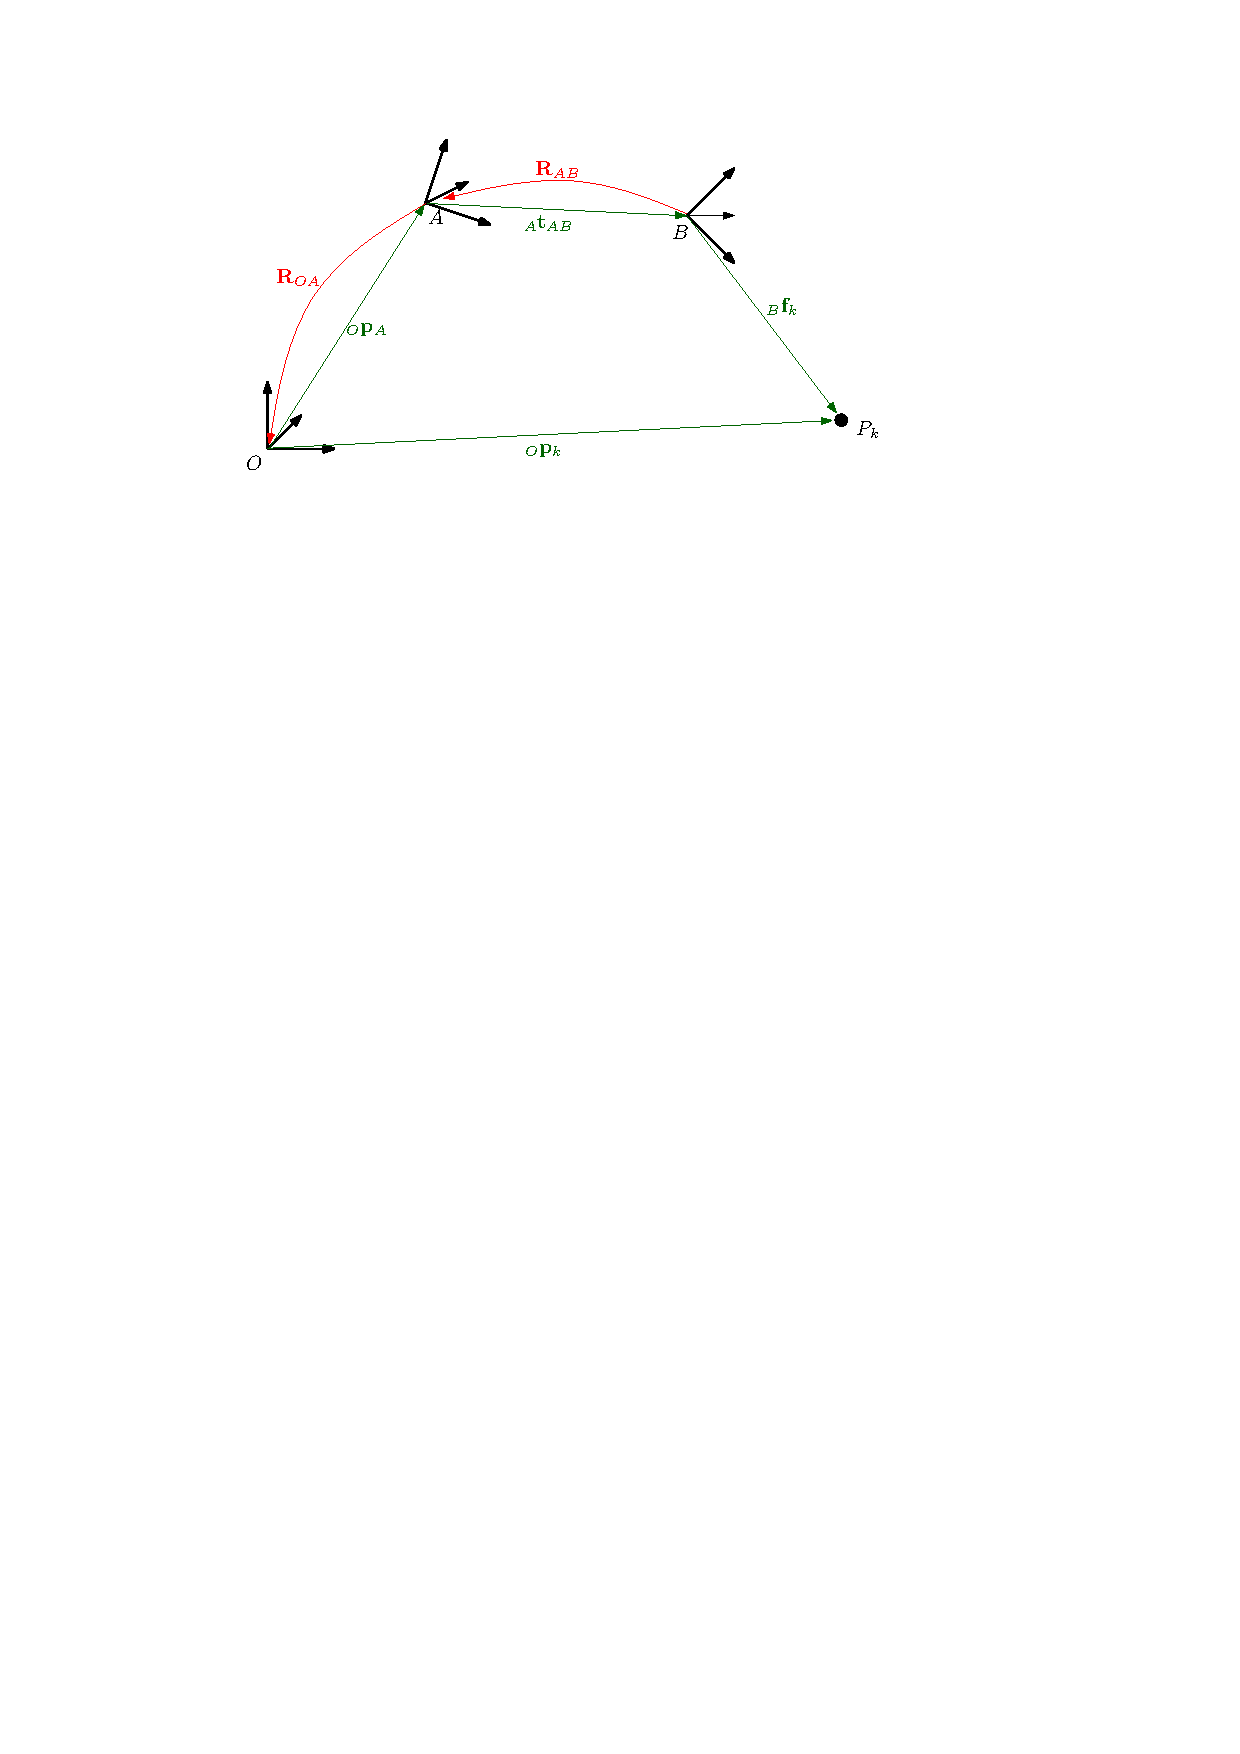
\includegraphics[width=0.6\textwidth]{img/notation.pdf}
     \caption{Example of a figure.}
     \label{img:notation}
  \end{figure}

\section{Including Matlab Figures}

When including figures into your report you want them as a vector graphic such that you can zoom into the figure without getting blurry.
Furthermore it is nice when the text in the figure gets substituted by \LaTeX\ such that you have the same font and the same font size.
Figure \ref{fig:example_tikz_figure} shows an example of such an imported matlab figure.
An easy way of achieving this is by using the \texttt{matlab2tikz} script.
You can find a short example on how to use this script in the \texttt{matlab\_figures} folder.
The \texttt{create\_figures.m} script creates a plot and then the tikz file which you can include in your document.
For using tikz, you need to make use of the \texttt{pgfplots} package in your \TeX\ document.
More information on using \texttt{matlab2tikz} can be found on \href{http://www.mathworks.com/matlabcentral/fileexchange/22022-matlab2tikz}{Matlab Central} where you can also download the necessary files (\texttt{matlab2tikz.m}, \texttt{matlab2tikzInputParser.m}, \texttt{updater.m}).

\begin{figure}[H]
  \centering
  \setlength\fwidth{8.0cm}
  \setlength\fheight{6.0cm}
  % This file was created by matlab2tikz v0.4.7 running on MATLAB 8.0.
% Copyright (c) 2008--2014, Nico Schlömer <nico.schloemer@gmail.com>
% All rights reserved.
% Minimal pgfplots version: 1.3
% 
% The latest updates can be retrieved from
%   http://www.mathworks.com/matlabcentral/fileexchange/22022-matlab2tikz
% where you can also make suggestions and rate matlab2tikz.
% 
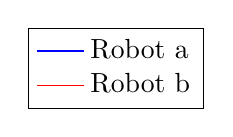
\begin{tikzpicture}

\begin{axis}[%
width=\fwidth,
height=\fheight,
scale only axis,
xmin=0,
xmax=10,
xlabel={time [$s$]},
ymin=-1,
ymax=1,
ylabel={velocity [$\frac{m}{s}$]},
legend style={draw=black,fill=white,legend cell align=left}
]
\addplot [color=blue,solid]
  table[row sep=crcr]{0	0\\
0.101010101010101	0.100838420258105\\
0.202020202020202	0.200648856522685\\
0.303030303030303	0.298413804447641\\
0.404040404040404	0.39313661214833\\
0.505050505050505	0.483851640437935\\
0.606060606060606	0.569634106908966\\
0.707070707070707	0.649609513505707\\
0.808080808080808	0.72296256147946\\
0.909090909090909	0.788945462844257\\
1.01010101010101	0.846885563602983\\
1.11111111111111	0.896192201029956\\
1.21212121212121	0.936362725104285\\
1.31313131313131	0.9669876227093\\
1.41414141414141	0.987754692360084\\
1.51515151515152	0.998452226900389\\
1.61616161616162	0.998971171723357\\
1.71717171717172	0.98930623651434\\
1.81818181818182	0.969555949182324\\
1.91919191919192	0.939921651430131\\
2.02020202020202	0.900705446202955\\
2.12121212121212	0.852307117939675\\
2.22222222222222	0.795220057023049\\
2.32323232323232	0.730026229976446\\
2.42424242424242	0.657390246682775\\
2.52525252525253	0.578052585106573\\
2.62626262626263	0.492822042588923\\
2.72727272727273	0.402567490669497\\
2.82828282828283	0.308209017490077\\
2.92929292929293	0.210708548077192\\
3.03030303030303	0.11106003812413\\
3.13131313131313	0.0102793412405343\\
3.23232323232323	-0.0906061470334077\\
3.33333333333333	-0.190567962875485\\
3.43434343434343	-0.288587058720432\\
3.53535353535354	-0.383664191806112\\
3.63636363636364	-0.474830110822239\\
3.73737373737374	-0.561155436815202\\
3.83838383838384	-0.641760137619388\\
3.93939393939394	-0.71582249922919\\
4.04040404040404	-0.782587502654202\\
4.14141414141414	-0.84137452086087\\
4.24242424242424	-0.89158425733514\\
4.34343434343434	-0.932704855531834\\
4.44444444444444	-0.964317116928778\\
4.54545454545455	-0.98609877449093\\
4.64646464646465	-0.997827777979213\\
4.74747474747475	-0.999384557612436\\
4.84848484848485	-0.990753243005677\\
4.94949494949495	-0.972021824958833\\
5.05050505050505	-0.943381258446\\
5.15151515151515	-0.905123515950137\\
5.25252525252525	-0.857638610988052\\
5.35353535353535	-0.80141062216897\\
5.45454545454545	-0.737012758318913\\
5.55555555555556	-0.665101514978822\\
5.65656565656566	-0.586409981847235\\
5.75757575757576	-0.501740369393911\\
5.85858585858586	-0.411955830830862\\
5.95959595959596	-0.317971662810619\\
6.06060606060606	-0.220745974555063\\
6.16161616161616	-0.121269920537167\\
6.26262626262626	-0.0205575962872592\\
6.36363636363636	0.0803642996702817\\
6.46464646464646	0.180466932359911\\
6.56565656565657	0.278729818677557\\
6.66666666666667	0.37415123057122\\
6.76767676767677	0.465758407025652\\
6.86868686868687	0.552617470746406\\
6.96969696969697	0.633842948448906\\
7.07070707070707	0.708606797699218\\
7.17171717171717	0.776146848283581\\
7.27272727272727	0.835774572052259\\
7.37373737373737	0.886882102029079\\
7.47474747474747	0.928948429231251\\
7.57575757575758	0.961544714026824\\
7.67676767676768	0.984338657883824\\
7.77777777777778	0.997097890943875\\
7.87878787878788	0.999692340886112\\
7.97979797979798	0.992095558932323\\
8.08080808080808	0.974384989475536\\
8.18181818181818	0.946741180583354\\
8.28282828282828	0.909445943424462\\
8.38383838383838	0.862879479381784\\
8.48484848484848	0.807516504139563\\
8.58585858585859	0.743921408256844\\
8.68686868686869	0.672742503562265\\
8.78787878787879	0.594705414024498\\
8.88888888888889	0.510605678474283\\
8.98989898989899	0.421300640588607\\
9.09090909090909	0.327700708813498\\
9.19191919191919	0.230760075325052\\
9.29292929292929	0.131466988642958\\
9.39393939393939	0.030833679061141\\
9.49494949494949	-0.0701139604006468\\
9.5959595959596	-0.170346832328096\\
9.6969696969697	-0.268843125910384\\
9.7979797979798	-0.364598733655889\\
9.8989898989899	-0.456637487633774\\
10	-0.54402111088937\\
};
\addlegendentry{Robot a};

\addplot [color=red,solid]
  table[row sep=crcr]{0	1\\
0.101010101010101	0.99490281585683\\
0.202020202020202	0.9796632259997\\
0.303030303030303	0.954436588420145\\
0.404040404040404	0.919480072752278\\
0.505050505050505	0.875150038590823\\
0.606060606060606	0.82189840263017\\
0.707070707070707	0.760268031659151\\
0.808080808080808	0.690887208377067\\
0.909090909090909	0.614463226448467\\
1.01010101010101	0.531775180091039\\
1.11111111111111	0.443666021702229\\
1.21212121212121	0.35103396849205\\
1.31313131313131	0.254823345726049\\
1.41414141414141	0.156014959925759\\
1.51515151515152	0.0556161001658067\\
1.61616161616162	-0.0453497306018852\\
1.71717171717172	-0.145853249514135\\
1.81818181818182	-0.244869886685079\\
1.91919191919192	-0.341390230048921\\
2.02020202020202	-0.434430315678286\\
2.12121212121212	-0.523041658674875\\
2.22222222222222	-0.606320922373835\\
2.32323232323232	-0.683419127290403\\
2.42424242424242	-0.753550305929445\\
2.52525252525253	-0.815999515227557\\
2.62626262626263	-0.870130124945965\\
2.72727272727273	-0.915390307713636\\
2.82828282828283	-0.951318664558728\\
2.92929292929293	-0.97754892857964\\
3.03030303030303	-0.993813698804694\\
3.13131313131313	-0.999947166176124\\
3.23232323232323	-0.995886803868673\\
3.33333333333333	-0.981674004711079\\
3.43434343434343	-0.957453659212335\\
3.53535353535354	-0.923472678494476\\
3.63636363636364	-0.880077477189673\\
3.73737373737374	-0.827710441961886\\
3.83838383838384	-0.76690542165429\\
3.93939393939394	-0.69828228503756\\
4.04040404040404	-0.62254060163933\\
4.14141414141414	-0.54045251007479\\
4.24242424242424	-0.452854846581271\\
4.34343434343434	-0.360640614001448\\
4.44444444444444	-0.264749878183483\\
4.54545454545455	-0.166160184603552\\
4.64646464646465	-0.0658765929072468\\
4.74747474747475	0.0350785690386048\\
4.84848484848485	0.135676127132719\\
4.94949494949495	0.234890552819178\\
5.05050505050505	0.331710417703216\\
5.15151515151515	0.425148704424772\\
5.25252525252525	0.514252868676963\\
5.35353535353535	0.598114549793553\\
5.45454545454545	0.67587883091213\\
5.55555555555556	0.746752954311448\\
5.65656565656566	0.810014403075603\\
5.75757575757576	0.865018266697566\\
5.85858585858586	0.911203815534403\\
5.95959595959596	0.948100217091764\\
6.06060606060606	0.975331335863734\\
6.16161616161616	0.992619567796701\\
6.26262626262626	0.999788670287321\\
6.36363636363636	0.996765558864523\\
6.46464646464646	0.983581052239521\\
6.56565656565657	0.960369558128524\\
6.66666666666667	0.927367703050975\\
6.76767676767677	0.884911920071669\\
6.86868686868687	0.833435019078179\\
6.96969696969697	0.773461774557475\\
7.07070707070707	0.705603575851525\\
7.17171717171717	0.630552194429187\\
7.27272727272727	0.54907273171308\\
7.37373737373737	0.461995819353901\\
7.47474747474747	0.37020915146548\\
7.57575757575758	0.274648435144047\\
7.67676767676768	0.176287851525489\\
7.77777777777778	0.0761301246240719\\
7.87878787878788	-0.0248037008054478\\
7.97979797979798	-0.125484668174093\\
8.08080808080808	-0.224886398621082\\
8.18181818181818	-0.321995554297938\\
8.28282828282828	-0.415822168707717\\
8.38383838383838	-0.505409738788067\\
8.48484848484848	-0.589844975855707\\
8.58585858585859	-0.668267116007629\\
8.68686868686869	-0.739876695065317\\
8.78787878787879	-0.80394369860703\\
8.88888888888889	-0.859815004003662\\
8.98989898989899	-0.906921038591359\\
9.09090909090909	-0.944781586105027\\
9.19191919191919	-0.973010682179788\\
9.29292929292929	-0.991320549013866\\
9.39393939393939	-0.99952452908148\\
9.49494949494949	-0.997538987988408\\
9.5959595959596	-0.985384167071799\\
9.6969696969697	-0.963183977052532\\
9.7979797979798	-0.931164734843692\\
9.8989898989899	-0.889652856392602\\
10	-0.839071529076452\\
};
\addlegendentry{Robot b};

\end{axis}
\end{tikzpicture}%
  \caption{Example figure created with \texttt{matlab2tikz}.}
  \label{fig:example_tikz_figure}
\end{figure}

An alternative which you might want to consider is \texttt{matlabfrag} and \texttt{mlf2pdf}.
Especially when there are many data points in your figure you might run into problems when using tikz.
Again, you can find a short example on how to use \texttt{mlf2pdf} in the \texttt{create\_figures.m} scriptin in the \texttt{matlab\_figures} folder.
This script makes use of the two functions \texttt{matlabfrag.m} and \texttt{mlf2pdf.m} to create a PDF which you can then include into matlab.
These two files can be downloaded \href{http://www.mathworks.ch/matlabcentral/fileexchange/28545-matlabfrag-to-pdf}{here} and \href{http://www.mathworks.ch/matlabcentral/fileexchange/21286-matlabfrag}{here}.

\begin{figure}[H]
     \centering
     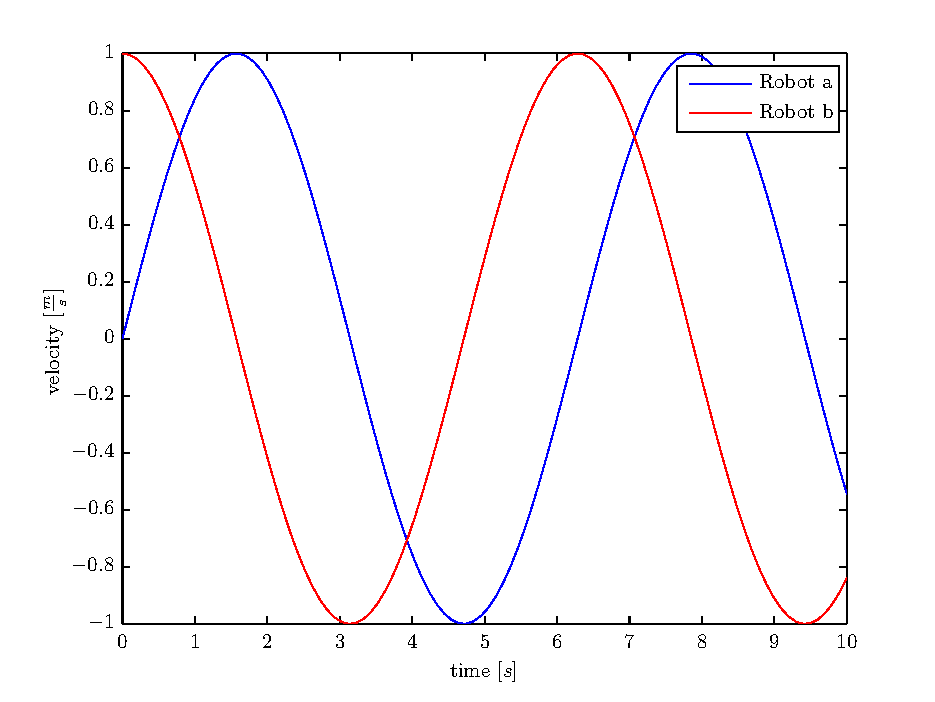
\includegraphics[width=0.85\textwidth]{matlab_figures/example_matlabfrag_figure.pdf}
     \caption{Example figure created with \texttt{mlf2pdf}.}
     \label{fig:example_matlab_fig}
  \end{figure}


\section{Including Code in your Document}

You may include samples from your Matlab code using the \texttt{lstlistings} environment, for example:

  \lstset{language=Matlab,numbers=none}
  \begin{lstlisting}[frame=lines, caption=Matlab Example, label=matlabexample]
  % Evaluate y = 2x
  for i = 1:length(x)

    y(i) = 2*x(i);

  end
  \end{lstlisting}

  \lstset{language=C++,numbers=none,caption=C++ Example, label=cppexample}
  \begin{lstlisting}[frame=lines]
  // sum all elements in a list
  int sum=0;
  for(list<int>::iterator it=mylist.begin(); it!=mylist.end(); ++it)
    sum += *it;
  \end{lstlisting}

\chapter{RPG Notation Style}\label{chap:notation}

This chapter presents some conventions on notation that we use at the Robotics and Perception Group.
Try to stick to those conventions since a unique style makes it easier to review the report.

\section{Variable styles in \LaTeX}

Use lowercase and bold letters for vectors, e.g. $\textbf{x}$, uppercase and bold letters for matrices, e.g. $\textbf{R}$, and lowercase letters with normal weight for scalars, e.g. $s$.

\section{Coordinate Systems and Rotations}

We use the notation introduced by Prof. Glocker in the course ``Mechanik 3'' at ETHZ to express coordinate frames, rotations and vectors.
Refer to Chapter~5 ``Kinematik'' in the lecture script for more details \footnote{\url{http://mitschriften.amiv.ethz.ch/main.php?page=3&scrid=1&pid=87&eid=1}}.
Figure \ref{fig:notation} gives an overview of how coordinate transformations and vectors are specified.
Observe that the coordinate system in which a vector is expressed is always written as index before the variable, e.g. $_B\mathbf{t}_{AB}$ is the vector from $A$ to $B$ expressed the coordinate system $B$.
For the ease of reading, the index for the origin coordinate frame can be omitted: $_O\mathbf{t}_k := \mathbf{t}_k$.

\begin{figure}[H]
     \centering
     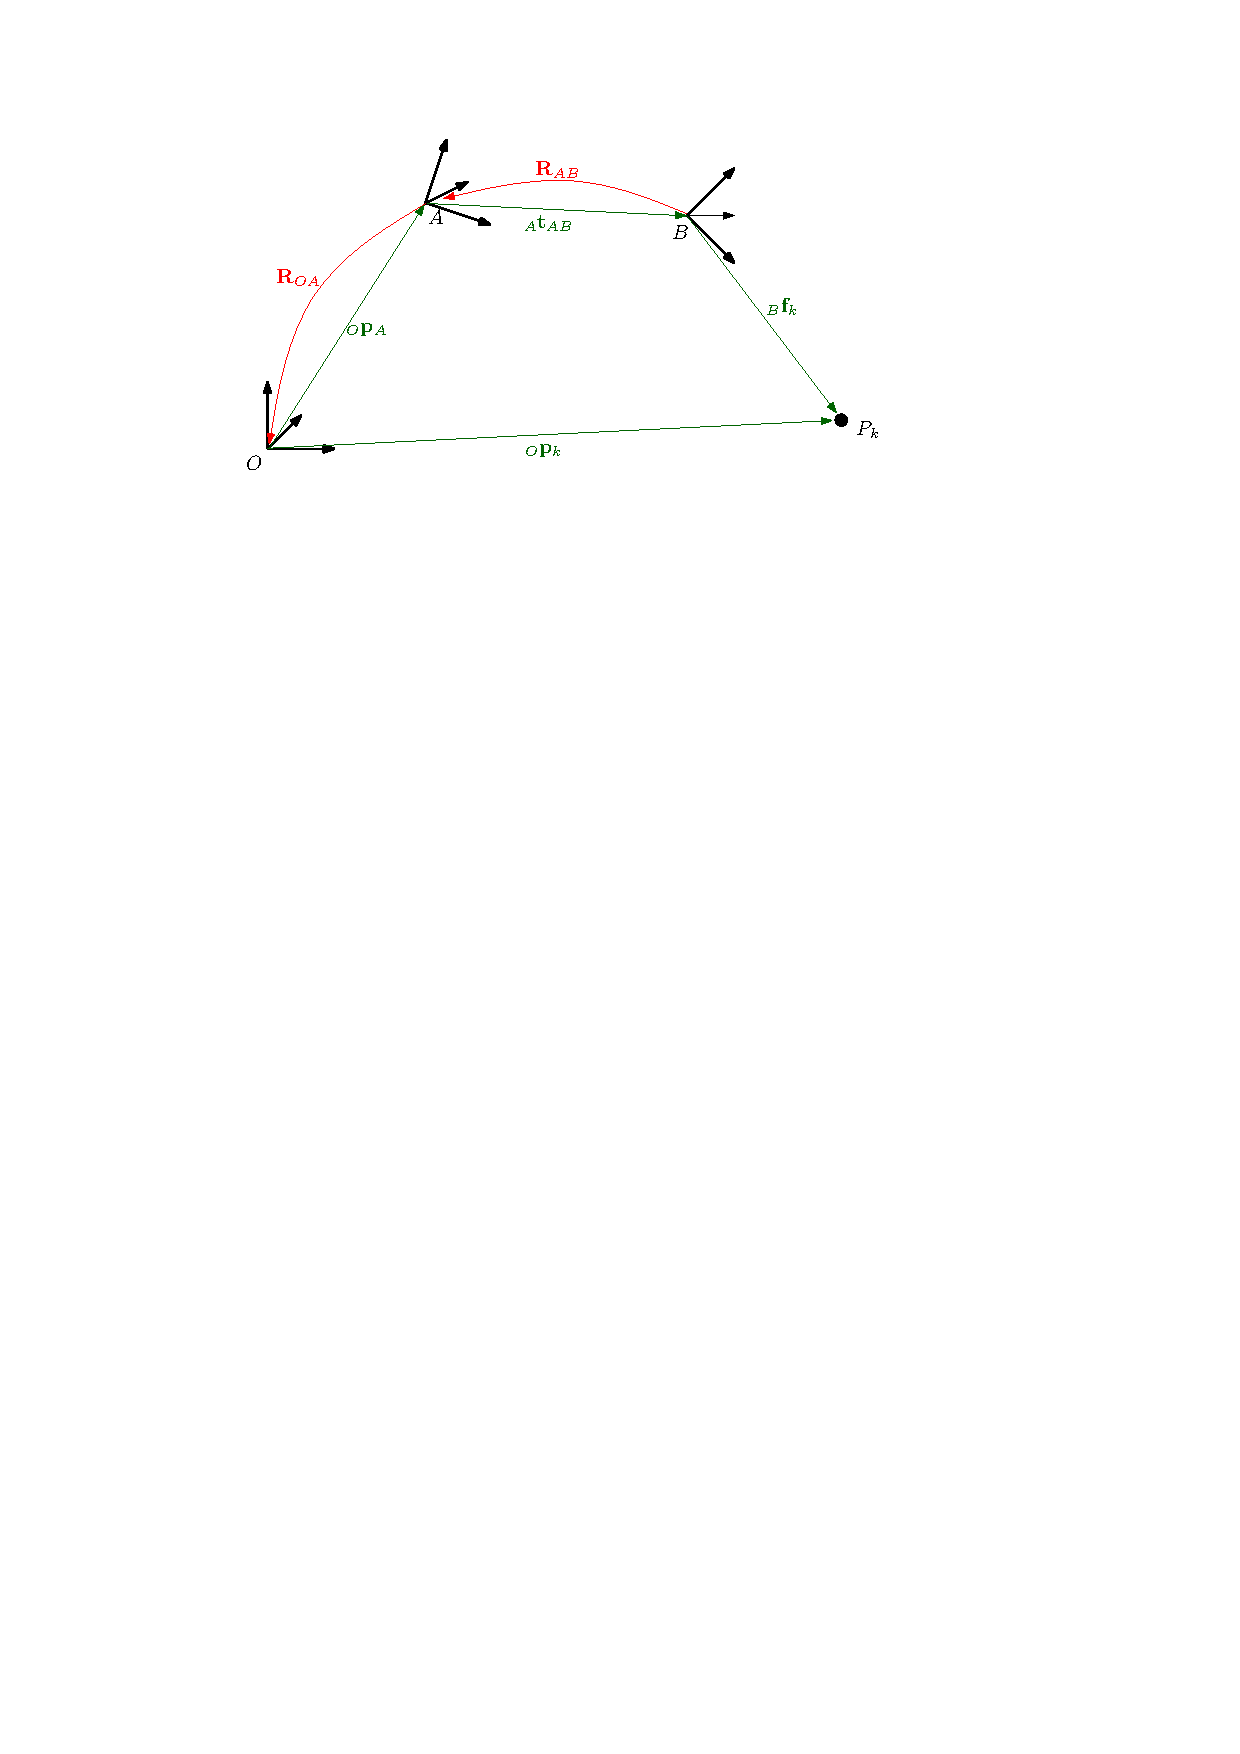
\includegraphics[scale=0.8]{img/notation}
     \caption{Notation overview.}
     \label{fig:notation}
\end{figure}
  
$A$ and $B$ are two adjacent coordinate frames and $O$ is the frame of origin.
$\mathbf{R}_{AB}$ describes the coordinate transformation from frame $B$ to frame $A$, thus it holds that 
	\[
		\begin{aligned}
			_O\mathbf{t}_k  &= \mathbf{R}_{OB} \ _B\mathbf{f}_k, \\
			\mathbf{R}_{OB} &= \mathbf{R}_{OA} \ \mathbf{R}_{AB}.
	  \end{aligned} 
	\]

\section{Measured, estimated and target values}

For controllers and estimators please specify the variables as follows in the report:

	\[
		\begin{aligned}
			\text{true value:} \quad & \mathbf{x} \\
			\text{estimated value:} \quad & \hat{\mathbf{x}} \\
			\text{measured value:} \quad & \tilde{\mathbf{x}} \\
			\text{desired value:} \quad & \mathbf{x}_\text{des} \\
      \text{error value:} \quad & \mathbf{x}_\text{e} \\
      \text{equilibrium value:} \quad & \mathbf{x}^* \\
		\end{aligned}
	\]

\chapter{Experiments}\label{chap:experiments}

Provide numerical results, plots, and timings. Interpret the data.

\begin{figure}[h]
   \centering
   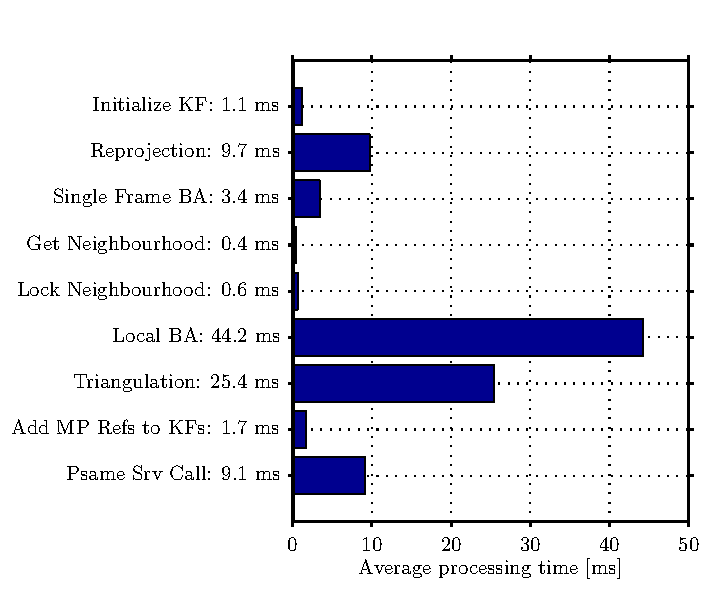
\includegraphics[width=0.75\textwidth]{img/processing_time.pdf}
   \caption{Example of a figure.}
   \label{img:timing}
\end{figure}
\chapter{Discussion}\label{chap:discussion}

Explain both the advantages and limitations of your approach.

\section{Conclusion}\label{sec:conclusion}

Summarize your work and what came out of it.

\section{Future Work}\label{sec:future_work}

How would you extend the work? Can you propose another approach?

\cleardoublepage

% Appendix______________________________________________________________________
\appendix

\chapter{Something}\label{sec:something}

In the appendix, you can provide some more data, a tutorial on how to run your code, a detailed proof, etc.

It is, however, not a requirement to have an appendix.

\cleardoublepage

% Bibliography__________________________________________________________________

\bibliographystyle{plain}
\bibliography{bibtex/references.bib}

\end{document}
